\documentclass{article}

\usepackage{fancyhdr}
\usepackage{extramarks}
\usepackage{amsmath}
\usepackage{hyperref}
\usepackage{amsthm}
\usepackage{amsfonts}
\usepackage{amssymb}
\usepackage{tikz}
\usepackage[plain]{algorithm}
\usepackage{algpseudocode}
\usepackage{diagbox}
\usepackage{gensymb}
\usepackage{comment}
\usepackage{float}
\usepackage{pifont}
\usepackage{graphicx}
\graphicspath{ {./images/}{../}{../../}{../../../}{./} }
\usepackage{bookmark}
\usepackage{multicol}
\setlength{\columnsep}{1cm}
\allowdisplaybreaks

\usetikzlibrary{automata,positioning}

%
% Basic Document Settings
%

\topmargin=-0.45in
\evensidemargin=0in
\oddsidemargin=0in
\textwidth=6.5in
\textheight=9.0in
\headsep=0.25in

\linespread{1.1}

\pagestyle{fancy}
\setlength{\headheight}{22.54448pt}
% \renewcommand{\sectionmark}[1]{
% \markboth{\thesection\quad #1}{}}
\fancyhead{}
\fancyhead[L]{\hmwkAuthorName\ \hmwkAuthorSID\\
\hmwkClass\hmwkClassTime\ (\hmwkClassInstructor): \hmwkTitle}
\fancyhead[C]{}
\fancyhead[R]{\rightmark}
\fancyfoot{}
\fancyfoot[C]{\thepage}

\renewcommand{\sectionmark}[1]{\markright{\thesection.\ #1}}

\renewcommand\headrulewidth{0.4pt}
\renewcommand\footrulewidth{0.4pt}

\setlength\parindent{0pt}

\newcommand{\fakesection}[1]{%
  \par\refstepcounter{section}% Increase section counter
  \sectionmark{#1}% Add section mark (header)
  \addcontentsline{toc}{section}{\protect\numberline{\thesection}#1}% Add section to ToC
  % Add more content here, if needed.
}

%
% Homework Details
%   - Title
%   - Due date
%   - Class
%   - Section/Time
%   - Instructor
%   - Author
%

\newcommand{\hmwkTitle}{Project Propoasl}
\newcommand{\hmwkDoneDate}{\today}
\newcommand{\hmwkClass}{AIST4010}
\newcommand{\hmwkClassTime}{}
\newcommand{\hmwkClassInstructor}{Prof. LI Yu}
\newcommand{\hmwkClassTitle}{Foundation of applied deep learning}
\newcommand{\hmwkAuthorName}{YUEN Yu Ching}
\newcommand{\hmwkAuthorSID}{1155143580}

\usepackage{hyperref}
\hypersetup{
    colorlinks=true,
    linkcolor=blue,
    filecolor=magenta,
    citecolor=teal,
    urlcolor=blue,
    pdftitle = {\hmwkClass\hmwkClassTime\ \hmwkTitle},
    pdfauthor = {\hmwkAuthorName \hmwkAuthorSID},
}
\urlstyle{same}

%
% Title Page
%

\title{AIST4010 Project Proposal}
\author{YUEN Yu Ching 1155143580}
\date{\today}

\renewcommand{\part}[1]{\textbf{\large Part \Alph{partCounter}}\stepcounter{partCounter}\\}

%
% Various Helper Commands
%

% Useful for algorithms
\newcommand{\alg}[1]{\textsc{\bfseries \footnotesize #1}}

% For derivatives
\newcommand{\deriv}[1]{\frac{\mathrm{d}}{\mathrm{d}x} (#1)}

% For partial derivatives
\newcommand{\pderiv}[2]{\frac{\partial}{\partial #1} (#2)}

% Integral dx
\newcommand{\dx}{\mathrm{d}x}

% Alias for the Solution section header
\newcommand{\solution}{\textbf{\large Solution}}

%Probability
\newcommand{\prob}[1]{\mathrm{P(}\textrm{#1}\mathrm{)}}

% Probability commands: Expectation, Variance, Covariance, Bias
\newcommand{\E}{\mathrm{E}}
\newcommand{\Var}{\mathrm{Var}}
\newcommand{\Cov}{\mathrm{Cov}}
\newcommand{\Bias}{\mathrm{Bias}}
\newcommand{\Or}{\textnormal{ or }}

\begin{document}
\maketitle
% \begin{multicols}{2}
\section{Project Goal}
In this project, we will be investigating the problem of anime posture transfer. Specifically, we will attempt to fine-tune a diffusion model such that given reference image of an anime character A and an image with an arbiturary character in pose B, the model will generate an image of character A in pose B.

\section{Significance of the project}
The anime industry in East Asian countries are having in increasingly large influence across the globe. Considering the heavy workload for desinging anime-esque characters, automating the generation of posing pictures of such characters could not only represent a reduction in cost, but also help creators get a better feel of their characters.

\section{Dataset}
We will be using a subset of the \href{https://gwern.net/danbooru2021}{Danbooru2021} \cite{danbooru2021} dataset. It is an extensive anime image dataset collected from the anime image aggregator Danbooru.\\

\begin{figure}
\centering
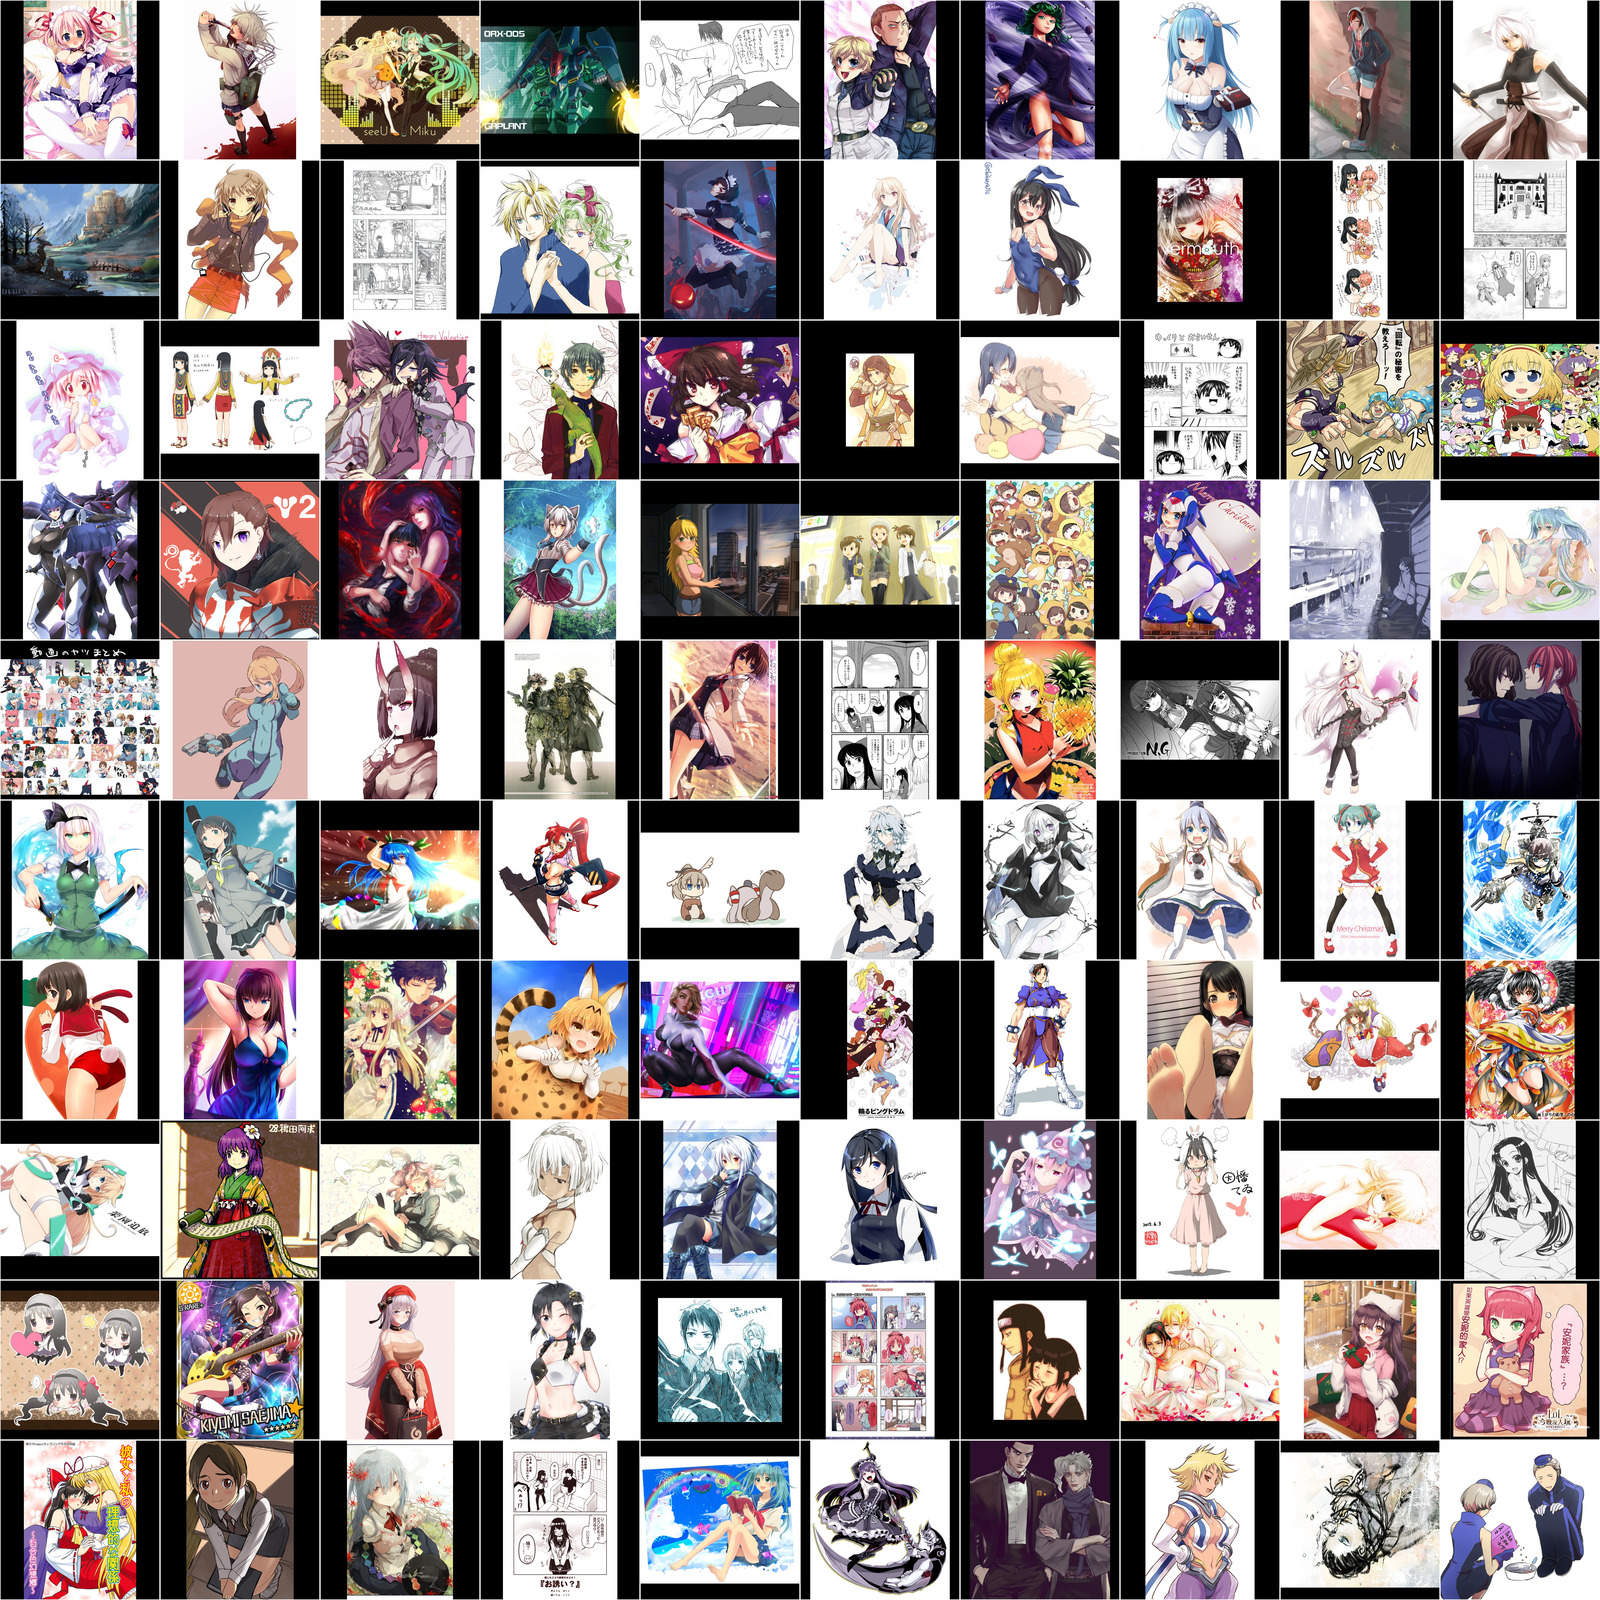
\includegraphics[scale=0.1]{danbooru2020-512px-samples.jpg}
\caption{100 sample images from the danbooru2021 dataset}
\end{figure}

The dataset in its totality is around 4.5 terabytes in size. However, as part of the project, we will be choosing a small subset of suitable images for training, and we expect it to be around 100 gigabytes after filtering.\\
However, we may face disk quota issues even with this reduced size. In such case, we will further refine the filter parameters until the working dataset is reduced to a reasonable size.

\section{Proposed method}
Given that we will be primarily working with anime images, we plan to fine-tune the \texttt{waifu-diffusion} diffusion model provided by hakurei on huggingface \cite{waifu-diffusion}. We plan to fine-tune it using ControlNet to ensure the validity of the final model.\\

\section{Related works}
There are similar models on feature transferral such as \cite{9050061}, which is based on GAN. Should there be enough time, we will attempt to compare the performance of the two architectures by separately training a GAN-based pose transerral model based on the findings in \cite{9050061}.

How will you evaluate your results? Qualitatively, what kind of results do you expect (e.g.,plots or figures)? Quantitatively, what kind of analysis will you use to evaluate and/or compare your results (e.g., what performance metrics or statistical tests)? What is your hypothesis regarding your results compared to baselines?
\section{Expected results}
Qualitatively, we will evaluate it using plots of its training loss and testing loss, as well as periodically generating testing samples to ensure that the training is progressing towards the objective.\\
Quantitavily, we will test various loss functions such as L1 loss and L2 loss for their efficicency in training, as proposed by Rogge and Rasul \cite{annotated-diffusion}.\\
We hypothesise that the results will be more detailed and accurate compared to baseline, as the training process will enable the model to recognize and utilize more features from the input images.
% \end{multicols}

\bibliographystyle{IEEEtran}
\bibliography{proposal}

\end{document}
